% fig:architecture — CRefNet-style pipeline for our model, with the supervised losses.
% Thumbnails: tests/viz/gen_arch_thumbs.py (data-only model), images/arch/*.png.
\begin{figure}[p]
  \centering
  \resizebox{\textwidth}{!}{%
  \begin{tikzpicture}[
      font=\sffamily, >=latex,
      thumb/.style={inner sep=0pt, draw=black!55, line width=0.4pt},
      blk/.style={draw=black!45, rounded corners=2pt, align=center, minimum height=15mm,
                  minimum width=12mm, line width=0.5pt, font=\small},
      dino/.style={blk, fill=teal!16, draw=teal!55, minimum height=30mm},
      dpt/.style={blk, fill=myblue!14, draw=myblue!55, minimum height=30mm},
      head/.style={blk, fill=orange!16, draw=orange!60},
      resid/.style={blk, fill=black!12, draw=black!50, minimum width=30mm},
      loss/.style={draw=red!55!black, circle, fill=red!7, inner sep=1pt, minimum size=8.5mm,
                   font=\footnotesize, text=red!60!black},
      io/.style={align=center, font=\small},
      dim/.style={font=\scriptsize\itshape, text=black!55, align=center},
      flow/.style={->, line width=0.8pt, black!70},
      lossflow/.style={->, line width=0.6pt, red!55!black},
      skipC/.style={->, line width=0.9pt, red!62!black, dashed},
      skipL/.style={->, line width=0.9pt, black!55, dash pattern=on 3pt off 2pt},
    ]
    % rows: albedo (top, y=+11), trunk (mid, y=0), shading (bottom, y=-11)
    % ── encoder + decoder (mid row) ─────────────────────────────────
    \node[thumb] (imgT) at (0,0) {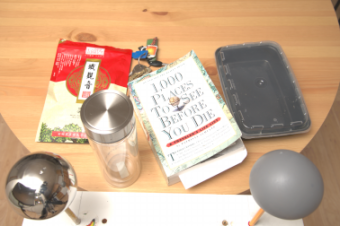
\includegraphics[width=19mm]{images/arch/input.png}};
    \node[io, above=0.5mm of imgT] {Input $\mathbf{I}$};
    \node[dino, right=9mm of imgT] (dino) {DINOv2-L/14\\[2pt]\emph{frozen}\\[2pt]{\scriptsize 4 stages, $\mathrm{d}{=}1024$}};
    \node[dim, above=0.4mm of dino] {material tokens};
    \node[dpt, right=10mm of dino] (dpt) {DPT\\decoder};
    \node[dim, below=0.5mm of dpt] {$768{\to}384{\to}192{\to}96{\to}64$};

    % ── heads (top / bottom rows) ───────────────────────────────────
    \node[head, above right=7mm and 12mm of dpt] (ah) {Albedo\\head};
    \node[head, below right=7mm and 12mm of dpt] (sh) {Shading\\head};

    % ── outputs + thumbnails ────────────────────────────────────────
    \node[io, right=8mm of ah] (Asym) {$\mathbf{A}\!\in\![0,1]^3$};
    \node[thumb, right=2.5mm of Asym] (albT) {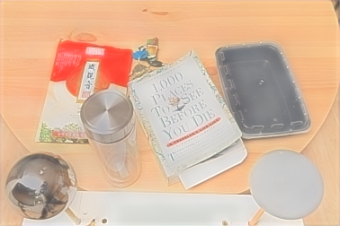
\includegraphics[width=15mm]{images/arch/albedo.png}};
    \node[io, right=8mm of sh] (Ssym) {$\boldsymbol{\pi}\!\in\!(0,1)^3$\\[1pt]$\mathbf{S}_d{=}\tfrac{1-\boldsymbol{\pi}}{\boldsymbol{\pi}}$};
    \node[thumb, right=2.5mm of Ssym] (shaT) {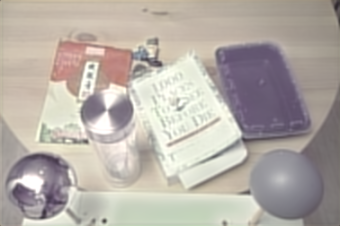
\includegraphics[width=15mm]{images/arch/shading.png}};

    % ── analytic residual: MUST sit downstream (right) of albT/shaT, since it is
    % computed FROM A and S_d. Placing it to their left (as an earlier draft did) forces
    % the A-> R and S_d->R arrows to run right-to-left, against the diagram's own
    % left-to-right reading order — that was the misleading part. Anchored off albT/shaT
    % themselves (not off dpt) so it automatically stays downstream of them.
    % Pin R's height EXACTLY to dpt/imgT's row (the guessed yshift offset in an earlier
    % draft was wrong). imgT, dino and dpt are chained with plain "right=" (no vertical
    % component), so they share one y; extracting x from albT.east and y from dpt.center
    % directly, via `let`, removes any guesswork about node-anchor offsets.
    \path let \p1 = ([xshift=20mm]albT.east), \p2 = (dpt.center) in
      node[resid] (R) at (\x1,\y2)
      {$\mathbf{R}{=}(\mathbf{I}{-}\mathbf{A}{\odot}\mathbf{S}_d)_{+}$\\[1pt]{\scriptsize analytic; \emph{no head}}};
    % Residual thumbnail sits to R's RIGHT (not below), on the way to its loss, mirroring
    % how albT/shaT sit between their heads and their own loss nodes.
    \node[thumb, right=6mm of R] (resT) {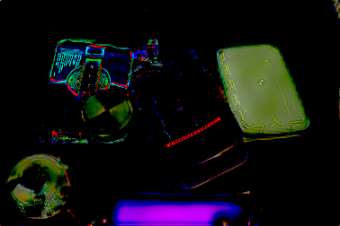
\includegraphics[width=13mm]{images/arch/residual.png}};

    % ── flows ───────────────────────────────────────────────────────
    \draw[flow] (imgT) -- (dino);
    \draw[flow] (dino) -- node[dim,above]{4 lvls} (dpt);
    \draw[flow] (dpt.east) -- ++(3mm,0) |- (ah.west);
    \draw[flow] (dpt.east) -- ++(3mm,0) |- (sh.west);
    \draw[flow] (ah) -- (Asym); \draw[flow] (Asym) -- (albT);
    \draw[flow] (sh) -- (Ssym); \draw[flow] (Ssym) -- (shaT);
    % A and S_d both feed R from the LEFT (upstream), arrowheads pointing right/down and
    % right/up INTO R — matches the left-to-right flow of the rest of the diagram.
    \draw[flow] (albT.south) -- ++(0,-4mm) -| (R.north);
    \draw[flow] (shaT.north) -- ++(0,4mm)  -| (R.south);

    % ── physics-typed skips ─────────────────────────────────────────
    \draw[skipC] (imgT.north) |- ([yshift=7mm]ah.north) -| (ah.north)
      node[dim,pos=0.25,above,text=red!55!black]{RGB skip $\mathbf{I}^{1/2.2}$ (3\,ch, colour)};
    \draw[skipL] (imgT.south) |- ([yshift=-7mm]sh.south) -| (sh.south)
      node[dim,pos=0.25,below]{luminance skip (1\,ch, intensity)};

    % ── SUPERVISED LOSSES (right column) ────────────────────────────
    \node[loss, right=10mm of albT] (la) {$\mathcal{L}_{\text{a}}$};
    \node[dim, right=0.5mm of la, text=red!55!black, align=left]
      {$+\,\mathcal{L}_{\text{msg-a}},\mathcal{L}_{\text{dssim}}$\\$+\,\mathcal{L}_{\text{chroma}},\mathcal{L}_{\text{mat}}$};
    \node[loss, right=10mm of shaT] (ls) {$\mathcal{L}_{\text{s}}$};
    \node[dim, right=0.5mm of ls, text=red!55!black, align=left]
      {$+\,\mathcal{L}_{\text{msg-s}},\mathcal{L}_{\text{sign}}$};
    % R.north = incoming A, R.south = incoming S_d (set above); R.east feeds the residual
    % thumbnail, which in turn feeds L_res — the same pattern albT->la and shaT->ls use.
    \node[loss, right=8mm of resT] (lr) {$\mathcal{L}_{\text{res}}$};
    \node[dim, above=0.3mm of lr, text=red!55!black]{sparsity $|\mathbf{R}|{\to}0$};

    \draw[lossflow] (albT) -- (la);
    \draw[lossflow] (shaT) -- (ls);
    \draw[flow] (R.east) -- (resT.west);
    \draw[lossflow] (resT.east) -- (lr);
    % CARI acts on the albedo too (training-only; detailed in fig:cari)
    \node[loss, above=4mm of la, draw=red!55!black, fill=red!7] (linv) {$\mathcal{L}_{\text{inv}}$};
    \node[dim, right=0.5mm of linv, text=red!55!black, align=left]{cross-render\\(\figref{fig:cari})};
    \draw[lossflow, dashed] (albT.north) to[bend left=12] (linv.west);

    % ── legend (own row, below everything) ──────────────────────────
    \coordinate (legY) at ([yshift=-24mm]sh.south -| imgT.west);
    \begin{scope}[shift={(legY)}]
      \node[dino, minimum height=5mm, minimum width=7mm] (l1) {};
      \node[io, right=1.5mm of l1] (l1t){frozen encoder};
      \node[dpt, minimum height=5mm, minimum width=7mm, right=7mm of l1t] (l2) {};
      \node[io, right=1.5mm of l2] (l2t){DPT decoder \scriptsize(trained)};
      \node[head, minimum height=5mm, minimum width=7mm, right=7mm of l2t] (l3) {};
      \node[io, right=1.5mm of l3] (l3t){output head \scriptsize(trained)};
      \node[loss, minimum size=6mm, right=8mm of l3t] (l4) {};
      \node[io, right=1.5mm of l4] (l4t){loss};
      \draw[skipC] ([xshift=8mm]l4t.east) -- ++(6mm,0);
      \node[io, right=1mm of l4t, xshift=14mm] (sc){colour skip};
      \draw[skipL] ([xshift=7mm]sc.east) -- ++(6mm,0);
      \node[io, right=13mm of sc]{intensity skip};
    \end{scope}
  \end{tikzpicture}}
  \caption[Model architecture and supervision.]{%
    Model architecture and its supervision. A \emph{frozen} DINOv2-Large encoder (teal)
    extracts patch features from four transformer stages; because it is never fine-tuned it
    supplies the illumination-invariant material tokens the backbone was pre-trained to
    produce, and only $18.5$M parameters downstream are learned. A DPT decoder (blue)
    reassembles and fuses the four levels into a shared full-resolution feature map. Two
    output heads (amber) read it, each with a \emph{physics-typed} full-resolution skip from
    the input: the albedo head takes the gamma-encoded RGB image (a colour path) and predicts
    $\mathbf{A}$; the shading head takes only the input luminance (an intensity path) and
    predicts the inverse shading $\boldsymbol{\pi}$, from which
    $\mathbf{S}_d=(1-\boldsymbol{\pi})/\boldsymbol{\pi}$ follows. The non-diffuse residual
    $\mathbf{R}=(\mathbf{I}-\mathbf{A}\odot\mathbf{S}_d)_{+}$ is analytic; there is no third
    head. Red nodes are the training losses on each output: the albedo family
    ($\mathcal{L}_{\text{a}}$ with its multi-scale-gradient, structural, chroma and
    material-consistency terms), the shading family ($\mathcal{L}_{\text{s}}$ with its
    gradient and sign terms), and a sparsity term $\mathcal{L}_{\text{res}}$ that pushes the
    analytic residual toward zero. The cross-render invariance loss $\mathcal{L}_{\text{inv}}$
    also constrains the albedo but acts across an illuminant pair at training time only
    (\figref{fig:cari}). Thumbnails are this model's own outputs on a MID test scene.
  }
  \label{fig:architecture}
\end{figure}
